\documentclass[tikz,border=5mm]{standalone}
\begin{document}
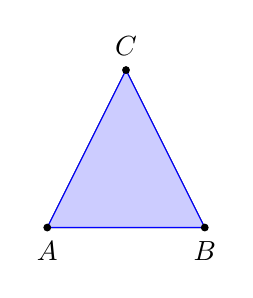
\begin{tikzpicture}
	\coordinate (A) at (0,0);
	\coordinate (B) at (2,0);
	\coordinate (C) at (1,2);
	
    % 绘制三角形外轮廓
    \draw (A) -- (B) -- (C) -- cycle;
    
    % 填充三角形
    \filldraw[fill=blue!20!white, draw=blue] (A) -- (B) -- (C) -- cycle;
    
    % 标注A、B、C
    \node [circle,fill=black,inner sep=1pt,label=below:$A$] at (A) {};
    \node [circle,fill=black,inner sep=1pt,label=below:$B$] at (B) {};
    \node [circle,fill=black,inner sep=1pt,label=above:$C$] at (C) {};
    
\end{tikzpicture}
\end{document}